% Native TikZ mechanism figures for Chapters 2 and 3.
% The diagrams use the document font and LaTeX font sizes instead of external
% PDF text, so they remain visually aligned with the thesis body.

\definecolor{ThesisInk}{HTML}{263241}
\definecolor{ThesisMuted}{HTML}{64748B}
\definecolor{ThesisBlue}{HTML}{2563EB}
\definecolor{ThesisBlueLight}{HTML}{DBEAFE}
\definecolor{ThesisTeal}{HTML}{0F766E}
\definecolor{ThesisTealLight}{HTML}{CCFBF1}
\definecolor{ThesisOrange}{HTML}{B45309}
\definecolor{ThesisOrangeLight}{HTML}{FEF3C7}
\definecolor{ThesisRed}{HTML}{B91C1C}
\definecolor{ThesisRedLight}{HTML}{FEE2E2}
\definecolor{ThesisGreen}{HTML}{15803D}
\definecolor{ThesisGreenLight}{HTML}{DCFCE7}
\definecolor{ThesisGray}{HTML}{E5E7EB}
\definecolor{ThesisGrayLight}{HTML}{F8FAFC}
\definecolor{ThesisViolet}{HTML}{6D28D9}
\definecolor{ThesisVioletLight}{HTML}{EDE9FE}

\tikzset{
  thesis box/.style={
    draw=ThesisInk!75,
    rounded corners=2pt,
    align=center,
    inner sep=3pt,
    minimum height=7mm,
    font=\footnotesize
  },
  thesis small box/.style={
    thesis box,
    font=\scriptsize,
    inner sep=2.5pt,
    minimum height=6mm
  },
  thesis arrow/.style={
    -{Latex[length=2.0mm,width=1.4mm]},
    draw=ThesisInk!75,
    line width=0.45pt
  },
  thesis mid arrow/.style={
    draw=ThesisInk!75,
    line width=0.45pt,
    postaction={decorate},
    decoration={
      markings,
      mark=at position 0.56 with {\arrow{Latex[length=2.0mm,width=1.4mm]}}
    }
  },
  thesis flow line/.style={
    draw=ThesisInk!75,
    line width=0.45pt
  },
  thesis soft line/.style={
    draw=ThesisMuted!55,
    line width=0.35pt
  },
  thesis axis/.style={
    -{Latex[length=2.0mm,width=1.4mm]},
    draw=ThesisInk,
    line width=0.45pt
  }
}

\newcommand{\figTheoryTaskResidency}{%
\begin{figure}[!ht]
\centering
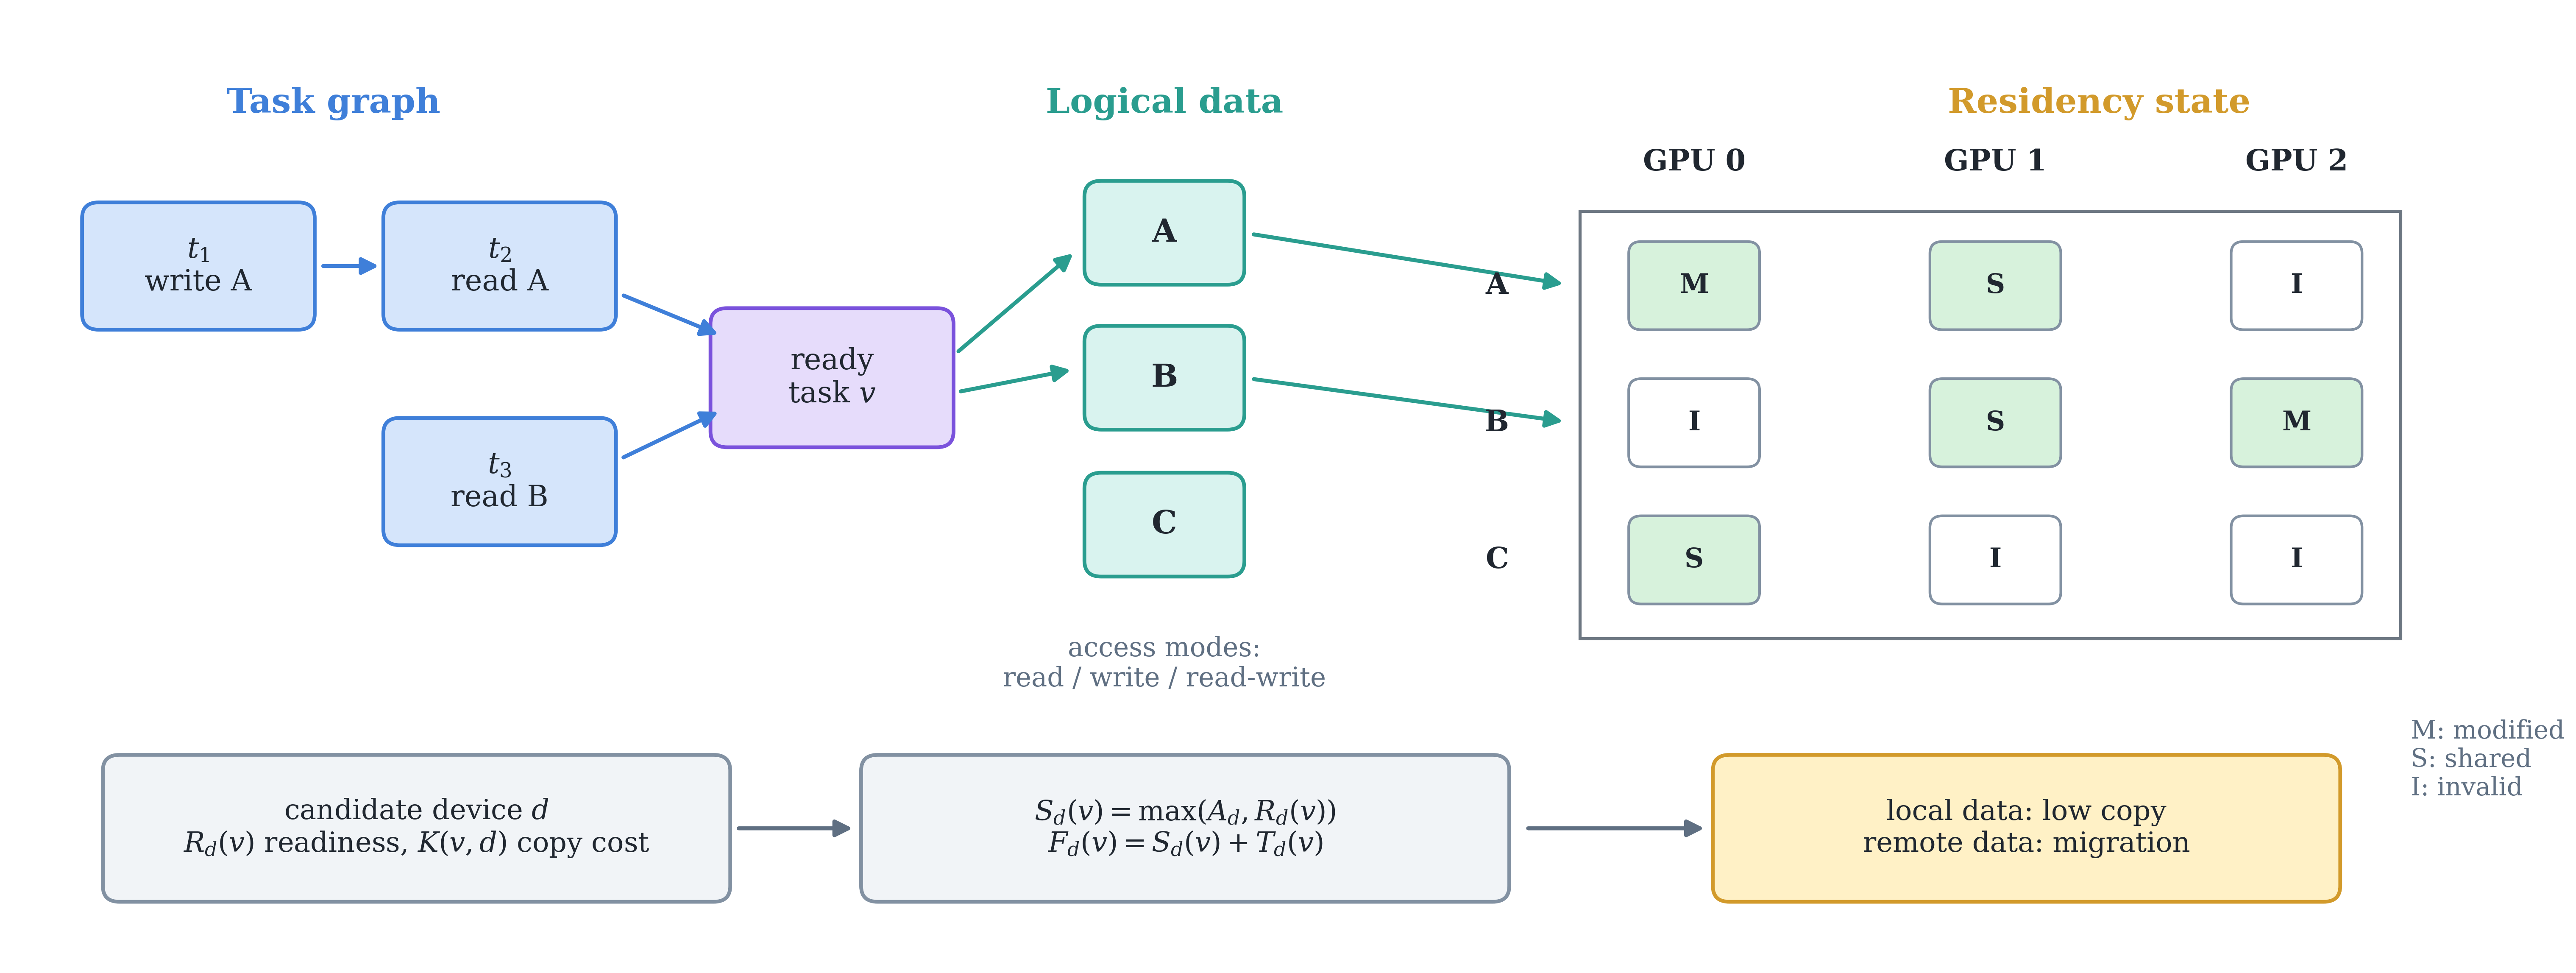
\includegraphics[width=0.88\linewidth,height=0.25\textheight,keepaspectratio]{figures/theory_task_residency.png}
\caption{CUDASTF task-graph execution model. Tasks form a DAG with data-driven dependencies, while each GPU maintains a changing view of logical data residency. Candidate placement decisions differ in device readiness, data-ready time, copy cost, and predicted finish time.}
\label{fig:theory-task-residency}
\end{figure}%
}

\newcommand{\figTheoryResidualGate}{%
\begin{figure}[!htbp]
\centering
\begin{tikzpicture}[x=1cm,y=1cm]
  \draw[thesis axis] (0,0) -- (10.7,0) node[below left=2pt and -12pt, font=\footnotesize] {normalized finish-time penalty $\rho_F$};
  \draw[thesis axis] (0,0) -- (0,5.0) node[above, font=\footnotesize] {normalized copy gain $\rho_K$};
  \foreach \x in {2,4,6,8,10} \draw[thesis soft line] (\x,0) -- (\x,4.65);
  \foreach \y in {1,2,3,4} \draw[thesis soft line] (0,\y) -- (10.4,\y);

  \fill[ThesisBlueLight] (0,1.25) rectangle (8.0,4.65);
  \draw[ThesisBlue, line width=0.7pt] (0,1.25) rectangle (8.0,4.65);
  \fill[ThesisTealLight] (0,2.65) rectangle (2.0,4.65);
  \draw[ThesisTeal, line width=0.8pt] (0,2.65) rectangle (2.0,4.65);

  \draw[ThesisBlue, dashed, line width=0.55pt] (8.0,0) -- (8.0,4.65);
  \draw[ThesisBlue, dashed, line width=0.55pt] (0,1.25) -- (10.4,1.25);
  \draw[ThesisTeal, dashed, line width=0.55pt] (2.0,0) -- (2.0,4.65);
  \draw[ThesisTeal, dashed, line width=0.55pt] (0,2.65) -- (10.4,2.65);

  \node[font=\scriptsize, text=ThesisBlue, align=center] at (6.8,4.35) {non-critical\\accepted region};
  \node[font=\scriptsize, text=ThesisTeal, align=center] at (1.0,4.35) {critical\\accepted};

  \node[circle, fill=ThesisTeal, inner sep=2.2pt, label={[font=\scriptsize,align=center]above right:accepted\\critical}] at (1.25,3.25) {};
  \node[circle, fill=ThesisBlue, inner sep=2.2pt, label={[font=\scriptsize,align=center]above right:accepted\\non-critical}] at (5.8,2.25) {};
  \node[circle, fill=ThesisOrange, inner sep=2.2pt, label={[font=\scriptsize,align=center]above right:copy gain\\too small}] at (4.2,0.75) {};
  \node[circle, fill=ThesisRed, inner sep=2.2pt, label={[font=\scriptsize,align=center]above right:penalty\\too large}] at (9.2,3.25) {};

  \node[font=\scriptsize, text=ThesisMuted] at (8.0,-0.32) {$\delta_{\mathrm{noncrit}}$};
  \node[font=\scriptsize, text=ThesisMuted] at (2.0,-0.32) {$\delta_{\mathrm{crit}}$};
  \node[font=\scriptsize, text=ThesisMuted, anchor=east] at (-0.08,2.65) {$\tau_{\mathrm{crit}}$};
  \node[font=\scriptsize, text=ThesisMuted, anchor=east] at (-0.08,1.25) {$\tau_{\mathrm{noncrit}}$};
\end{tikzpicture}
\caption{Acceptance region of the HEFT-relative residual gate. A non-HEFT candidate is accepted only when its normalized finish-time penalty remains below the active threshold and its normalized copy gain exceeds the required evidence threshold. Critical tasks use stricter gates than non-critical tasks.}
\label{fig:theory-residual-gate-region}
\end{figure}%
}

\newcommand{\figTheoryDvfsTimeline}{%
\begin{figure}[!ht]
\centering
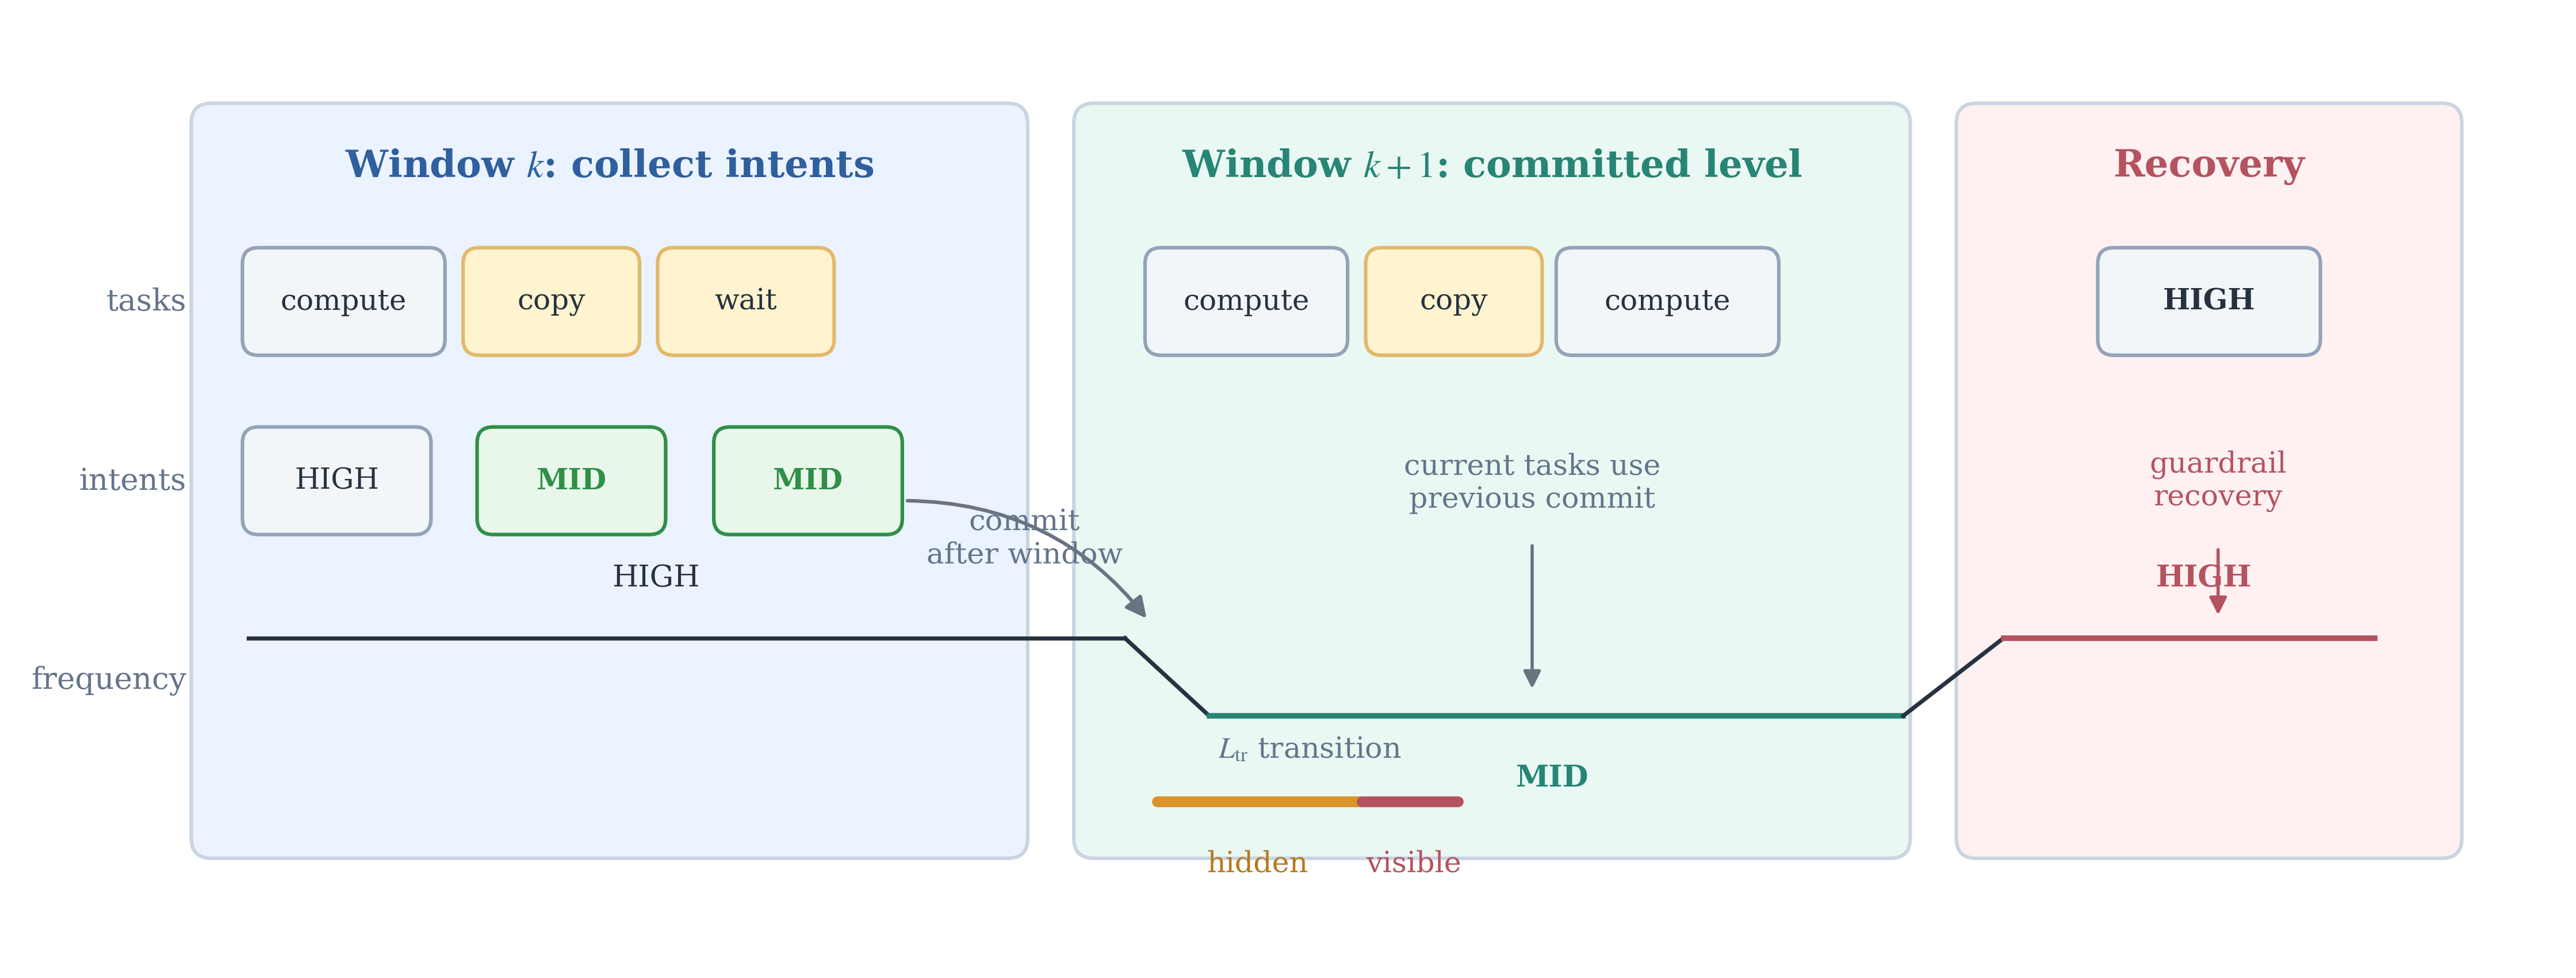
\includegraphics[width=0.90\linewidth,height=0.23\textheight,keepaspectratio]{figures/theory_dvfs_timeline.png}
\caption{Windowed proposal--commit DVFS and transition amortization. Task-level intents are accumulated over a per-GPU window, while the committed frequency level is applied to later tasks. Transition latency can be partially hidden by communication or slack.}
\label{fig:theory-dvfs-timeline}
\end{figure}%
}

\newcommand{\figMethodsRuntimePipeline}{%
\begin{figure}[!htbp]
\centering
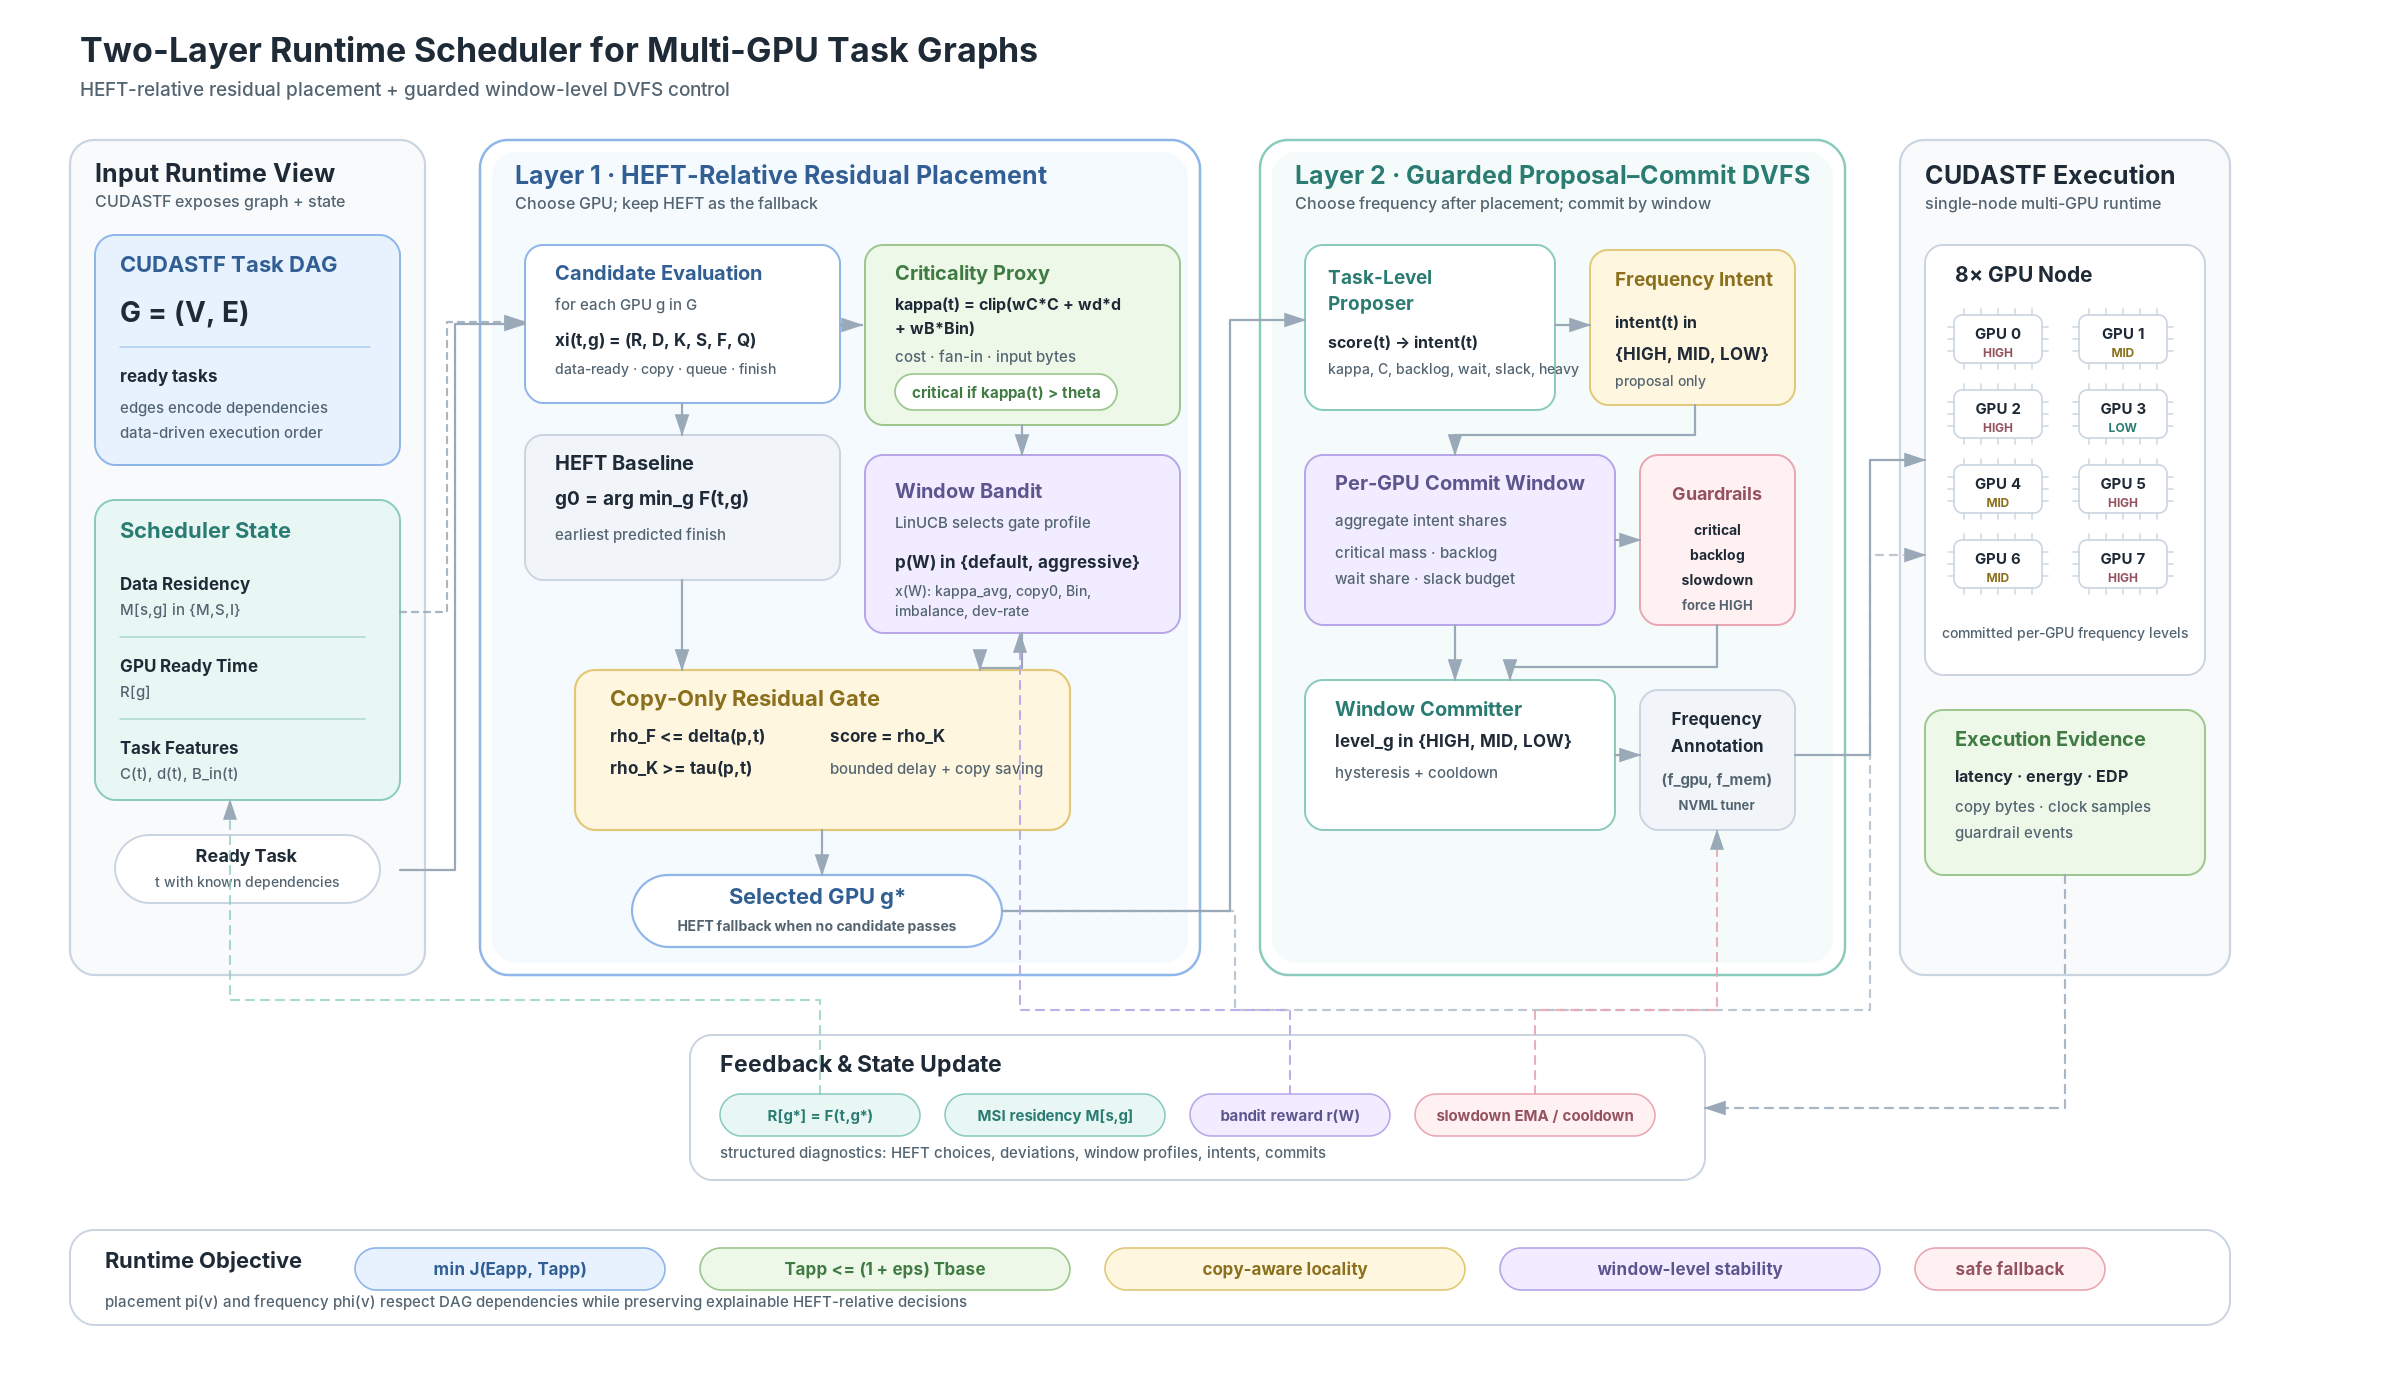
\includegraphics[width=\linewidth]{figures/system_overview.png}
\caption{Overview of the proposed two-layer runtime scheduler. CUDASTF exposes a task graph and runtime state to the placement layer, which applies a HEFT-relative residual gate. The selected GPU is then passed to the guarded proposal--commit DVFS layer, and execution feedback updates ready times, data residency, bandit rewards, and slowdown guardrails.}
\label{fig:methods-runtime-pipeline}
\end{figure}%
}

\newcommand{\figMethodsPlacementMotivation}{%
\begin{figure}[!ht]
\centering
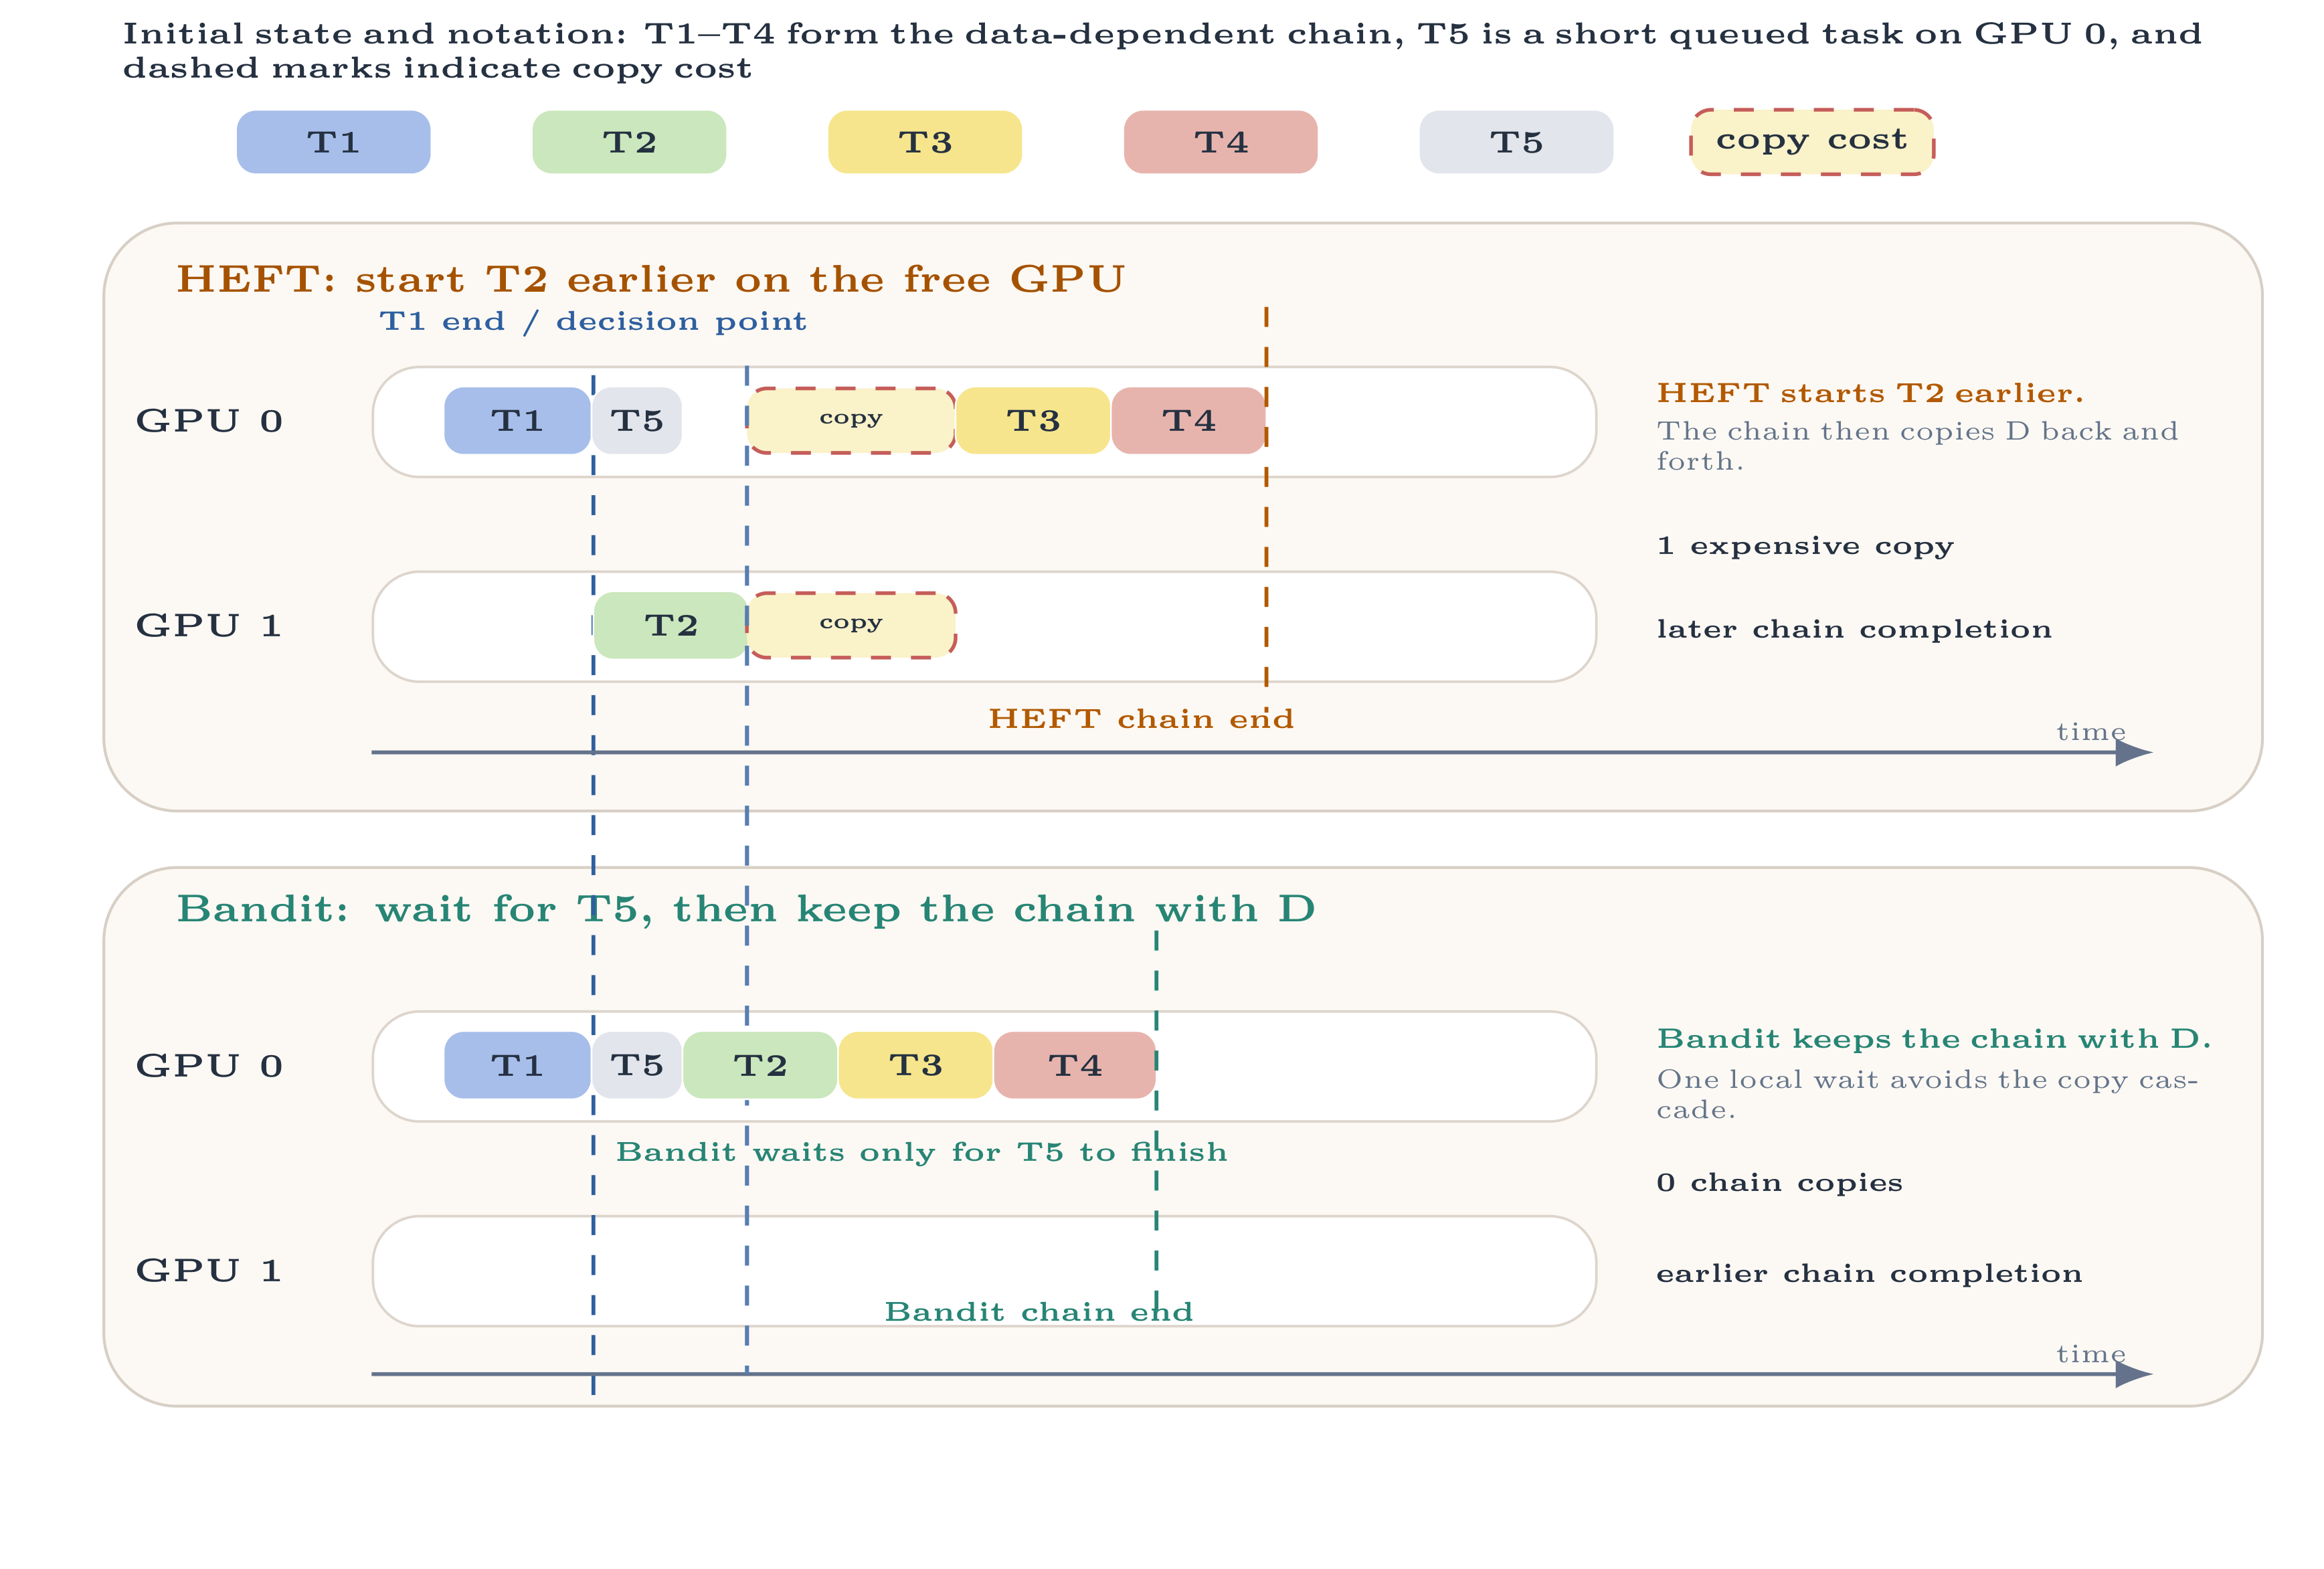
\includegraphics[width=0.82\linewidth,height=0.28\textheight,keepaspectratio]{figures/methods_placement_motivation.png}
\caption{Motivating example for HEFT-relative residual placement. A HEFT-local earliest-finish decision can introduce downstream copies, while a bounded residual deviation can keep successor data local.}
\label{fig:methods-placement-motivation}
\end{figure}%
}

\newcommand{\figMethodsResidualFlowTikz}{%
\begin{tikzpicture}[x=1cm,y=1cm]
  \node[thesis box, fill=ThesisGrayLight, text width=2.4cm] (task) at (5.7,7.15) {Ready task $t$};
  \node[thesis box, fill=ThesisBlueLight, draw=ThesisBlue, text width=5.2cm] (eval) at (5.7,5.95) {Select profile $p_W$ and\\evaluate all GPU candidates};
  \node[thesis box, fill=ThesisBlueLight, draw=ThesisBlue, text width=5.2cm] (base) at (5.7,4.70) {Choose HEFT baseline $g_0$\\and compute $q(t)$};
  \node[thesis box, fill=ThesisVioletLight, draw=ThesisViolet, text width=2.7cm] (crit) at (5.7,3.40) {$q(t)>\theta_q$?};
  \node[thesis box, fill=ThesisTealLight, draw=ThesisTeal, text width=2.7cm] (cg) at (2.25,1.55) {Critical gate\\small $\delta$, high $\tau$};
  \node[thesis box, fill=ThesisBlueLight, draw=ThesisBlue, text width=2.9cm] (ng) at (9.15,1.55) {Non-critical gate\\larger $\delta$, lower $\tau$};
  \node[thesis box, fill=ThesisOrangeLight, draw=ThesisOrange, text width=6.4cm] (filter) at (5.7,-0.02) {Filter candidates with $\rho_F\leq\delta$ and $\rho_K\geq\tau$};
  \node[thesis box, fill=ThesisGrayLight, text width=2.45cm] (heft) at (2.35,-1.34) {empty set:\\$g^*=g_0$};
  \node[thesis box, fill=ThesisGreenLight, draw=ThesisGreen, text width=3.15cm] (best) at (9.05,-1.34) {feasible set:\\$g^*=\arg\max H(t,g)$};
  \coordinate (cgEntry) at ($(cg.north)+(-0.70,0)$);
  \coordinate (ngEntry) at ($(ng.north)+(0.70,0)$);
  \coordinate (heftEntry) at ($(heft.north)+(-0.68,0)$);
  \coordinate (bestEntry) at ($(best.north)+(0.74,0)$);

  \draw[thesis arrow] (task.south) -- (eval.north);
  \draw[thesis arrow] (eval.south) -- (base.north);
  \draw[thesis arrow] (base.south) -- (crit.north);
  \coordinate (critSplit) at (5.7,2.62);
  \draw[thesis flow line] (crit.south) -- (critSplit);
  \draw[thesis arrow] (critSplit) -| (cgEntry);
  \draw[thesis arrow] (critSplit) -| (ngEntry);
  \node[font=\scriptsize, text=ThesisMuted] at (3.25,2.72) {yes};
  \node[font=\scriptsize, text=ThesisMuted] at (8.15,2.72) {no};
  \coordinate (gateMerge) at (5.7,0.72);
  \draw[thesis flow line] (cg.south) -- ++(0,-0.36) -| (gateMerge);
  \draw[thesis flow line] (ng.south) -- ++(0,-0.36) -| (gateMerge);
  \draw[thesis arrow] (gateMerge) -- (filter.north);
  \coordinate (filterSplit) at (5.7,-0.68);
  \draw[thesis flow line] (filter.south) -- (filterSplit);
  \draw[thesis arrow] (filterSplit) -| (heftEntry);
  \draw[thesis arrow] (filterSplit) -| (bestEntry);
  \node[font=\scriptsize, text=ThesisMuted, align=center] at (5.7,-2.34)
    {$H(t,g)=\rho_K(t,g)$ in the copy-only configuration};
\end{tikzpicture}
}

\newcommand{\figMethodsResidualFlow}{%
\begin{figure}[!htbp]
\centering
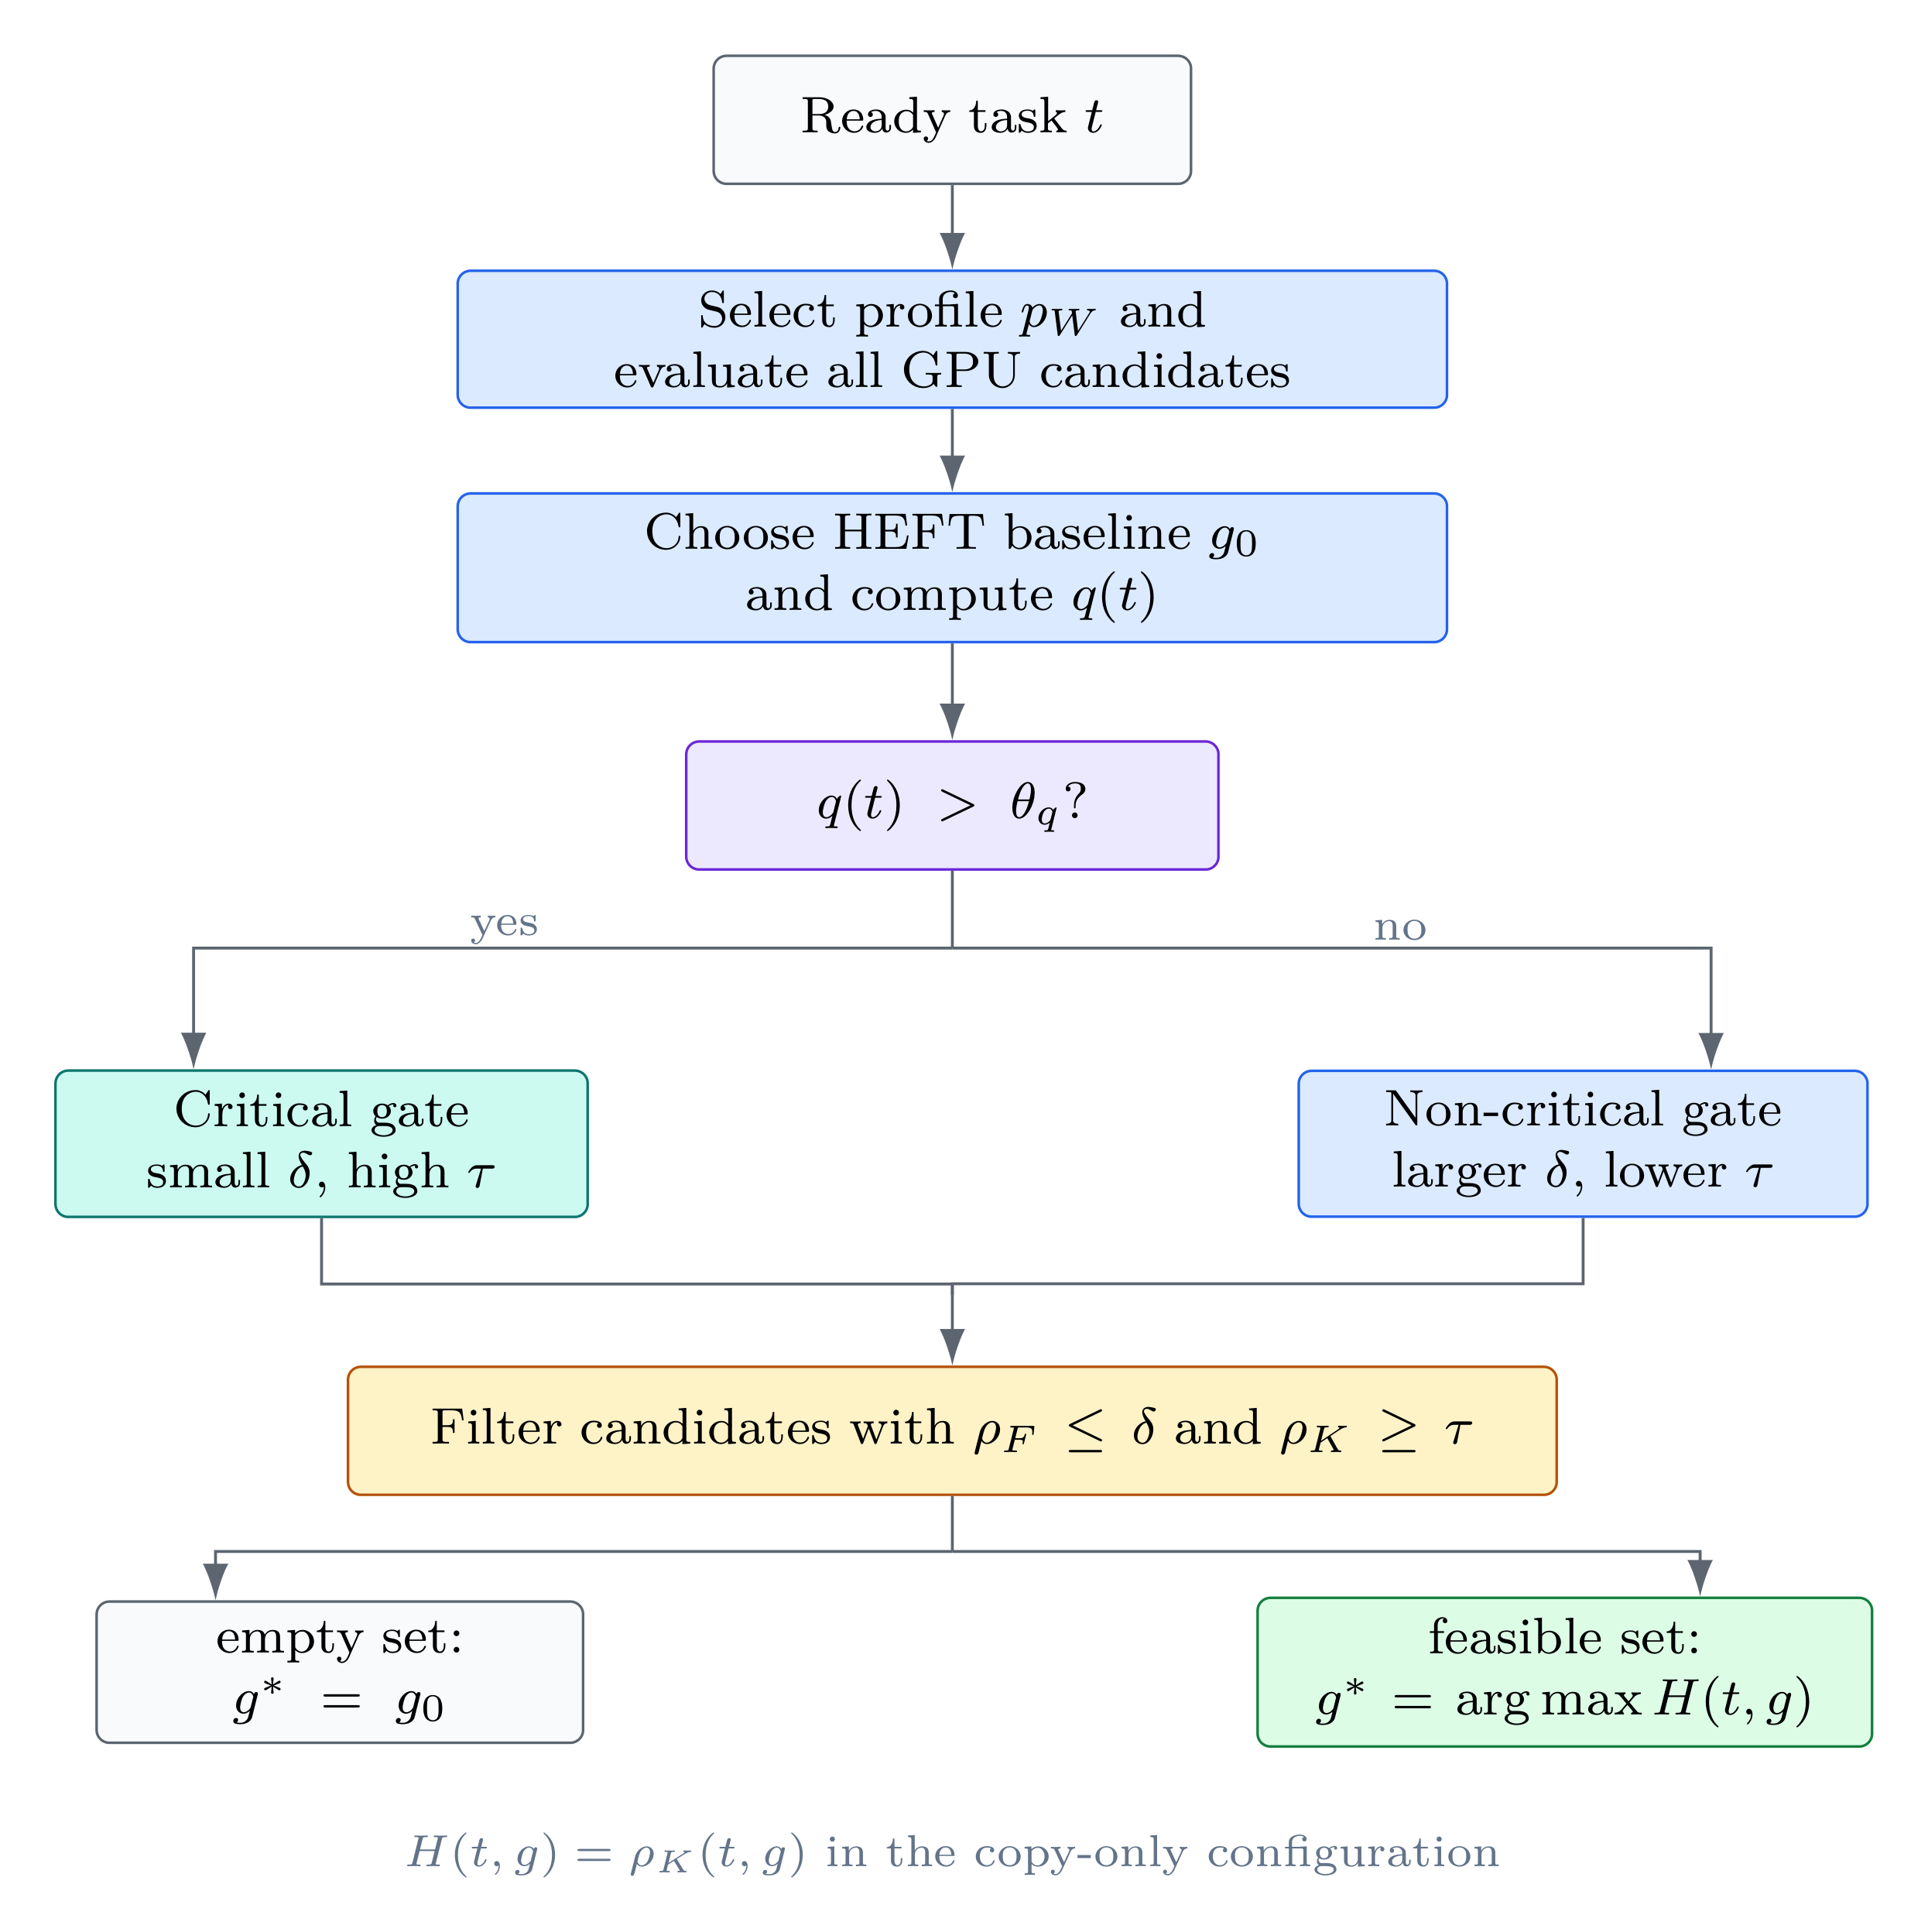
\includegraphics[width=0.78\linewidth,height=0.38\textheight,keepaspectratio]{figures/methods_residual_flow.png}
\caption{HEFT-relative residual placement decision. The scheduler accepts a non-baseline GPU only when the active profile's finish-time and copy-gain gates pass; otherwise it falls back to HEFT.}
\label{fig:methods-residual-flow}
\end{figure}%
}

\newcommand{\figMethodsBanditLoop}{%
\begin{figure}[!htbp]
\centering
\begin{tikzpicture}[x=1cm,y=1cm]
  \node[thesis box, fill=ThesisGrayLight, text width=2.25cm] (stats) at (1.30,4.30) {Completed window statistics};
  \node[thesis box, fill=ThesisBlueLight, draw=ThesisBlue, text width=2.20cm] (ctx) at (4.25,4.30) {Context vector\\$x(W)$};
  \node[thesis box, fill=ThesisBlueLight, draw=ThesisBlue, text width=2.05cm] (score) at (7.10,4.30) {LinUCB scores};
  \node[thesis box, fill=ThesisVioletLight, draw=ThesisViolet, text width=2.55cm] (profile) at (10.25,4.30) {Gate profile for next window};
  \node[thesis box, fill=ThesisGreenLight, draw=ThesisGreen, text width=2.55cm] (exec) at (8.65,2.25) {Residual gate executes tasks};
  \node[thesis box, fill=ThesisOrangeLight, draw=ThesisOrange, text width=2.10cm] (reward) at (5.20,2.25) {Relative reward};
  \node[thesis box, fill=ThesisOrangeLight, draw=ThesisOrange, text width=2.20cm] (update) at (1.30,2.25) {Update\\active arm};

  \draw[thesis arrow] (stats) -- (ctx);
  \draw[thesis arrow] (ctx) -- (score);
  \draw[thesis arrow] (score) -- (profile);
  \draw[thesis arrow] (profile.east) -- ++(0.45,0) |- (exec.east);
  \draw[thesis arrow] (exec) -- (reward);
  \draw[thesis arrow] (reward) -- (update);
  \draw[thesis arrow] (update.north) -- (stats.south);

  \node[font=\scriptsize, align=center, text=ThesisMuted] at (5.80,5.20)
    {$\overline{q}$, $\phi_{\mathrm{high}}$, $\overline{K}_0$, $\overline{B}_{\mathrm{in}}$, $\overline{d}$, $\overline{C}$, $\overline{L}_{\mathrm{imb}}$, $\phi_{\mathrm{dev}}$};
  \node[thesis small box, fill=ThesisRedLight, draw=ThesisRed, text width=3.05cm] at (8.65,0.92)
    {The bandit selects a profile, not a GPU.};
  \node[font=\scriptsize, text=ThesisOrange] at (5.20,1.35) {$r^{\mathrm{rel}}=r^{\mathrm{active}}-r^{\mathrm{default}}$};
\end{tikzpicture}
\caption{Window-level contextual-bandit adaptation. Window statistics form the context for the next scheduling window; LinUCB selects the residual-gate profile, and the selected profile is updated using relative reward after the window completes.}
\label{fig:methods-bandit-loop}
\end{figure}%
}

\newcommand{\figMethodsDvfsStateMachineTikz}{%
\begin{tikzpicture}[x=1cm,y=1cm]
  \node[font=\footnotesize\bfseries, text=ThesisTeal] at (1.85,4.65) {Task-level proposer};
  \node[font=\footnotesize\bfseries, text=ThesisViolet] at (5.25,4.65) {Per-GPU window};
  \node[font=\footnotesize\bfseries, text=ThesisBlue] at (9.35,4.65) {Committed level};

  \node[thesis small box, fill=ThesisTealLight, draw=ThesisTeal, text width=2.70cm] (proposer) at (1.85,3.35)
    {task features\\criticality, cost\\wait, slack\\intent: HIGH/MID/LOW};
  \node[thesis small box, fill=ThesisVioletLight, draw=ThesisViolet, text width=2.90cm] (window) at (5.25,3.35)
    {aggregate intents\\critical mass\\backlog and slack\\commit if stable};
  \node[thesis small box, fill=ThesisRedLight, draw=ThesisRed, text width=2.20cm] (guard) at (7.45,1.75)
    {guardrails\\slowdown\\or backlog};

  \node[thesis small box, fill=ThesisGrayLight, text width=1.15cm] (high) at (8.75,3.35) {HIGH};
  \node[thesis small box, fill=ThesisGreenLight, draw=ThesisGreen, text width=1.15cm] (mid) at (10.55,3.35) {MID};
  \node[thesis small box, fill=ThesisOrangeLight, draw=ThesisOrange, text width=1.15cm] (low) at (10.55,2.05) {LOW};

  \node[thesis small box, fill=ThesisGrayLight, text width=6.80cm] (note) at (5.75,0.62)
    {the current task uses the previously committed level;\\new intents affect a later window};

  \draw[thesis arrow] (proposer.east) -- (window.west);
  \draw[thesis arrow] (window.east) -- (high.west);
  \draw[thesis arrow, ThesisGreen] (high.east) -- (mid.west);
  \draw[thesis arrow, ThesisOrange] (mid.south) -- (low.north);
  \draw[thesis flow line, ThesisRed, dashed] (guard.north) -- (high.south);
\end{tikzpicture}
}

\newcommand{\figMethodsDvfsStateMachine}{%
\begin{figure}[!htbp]
\centering
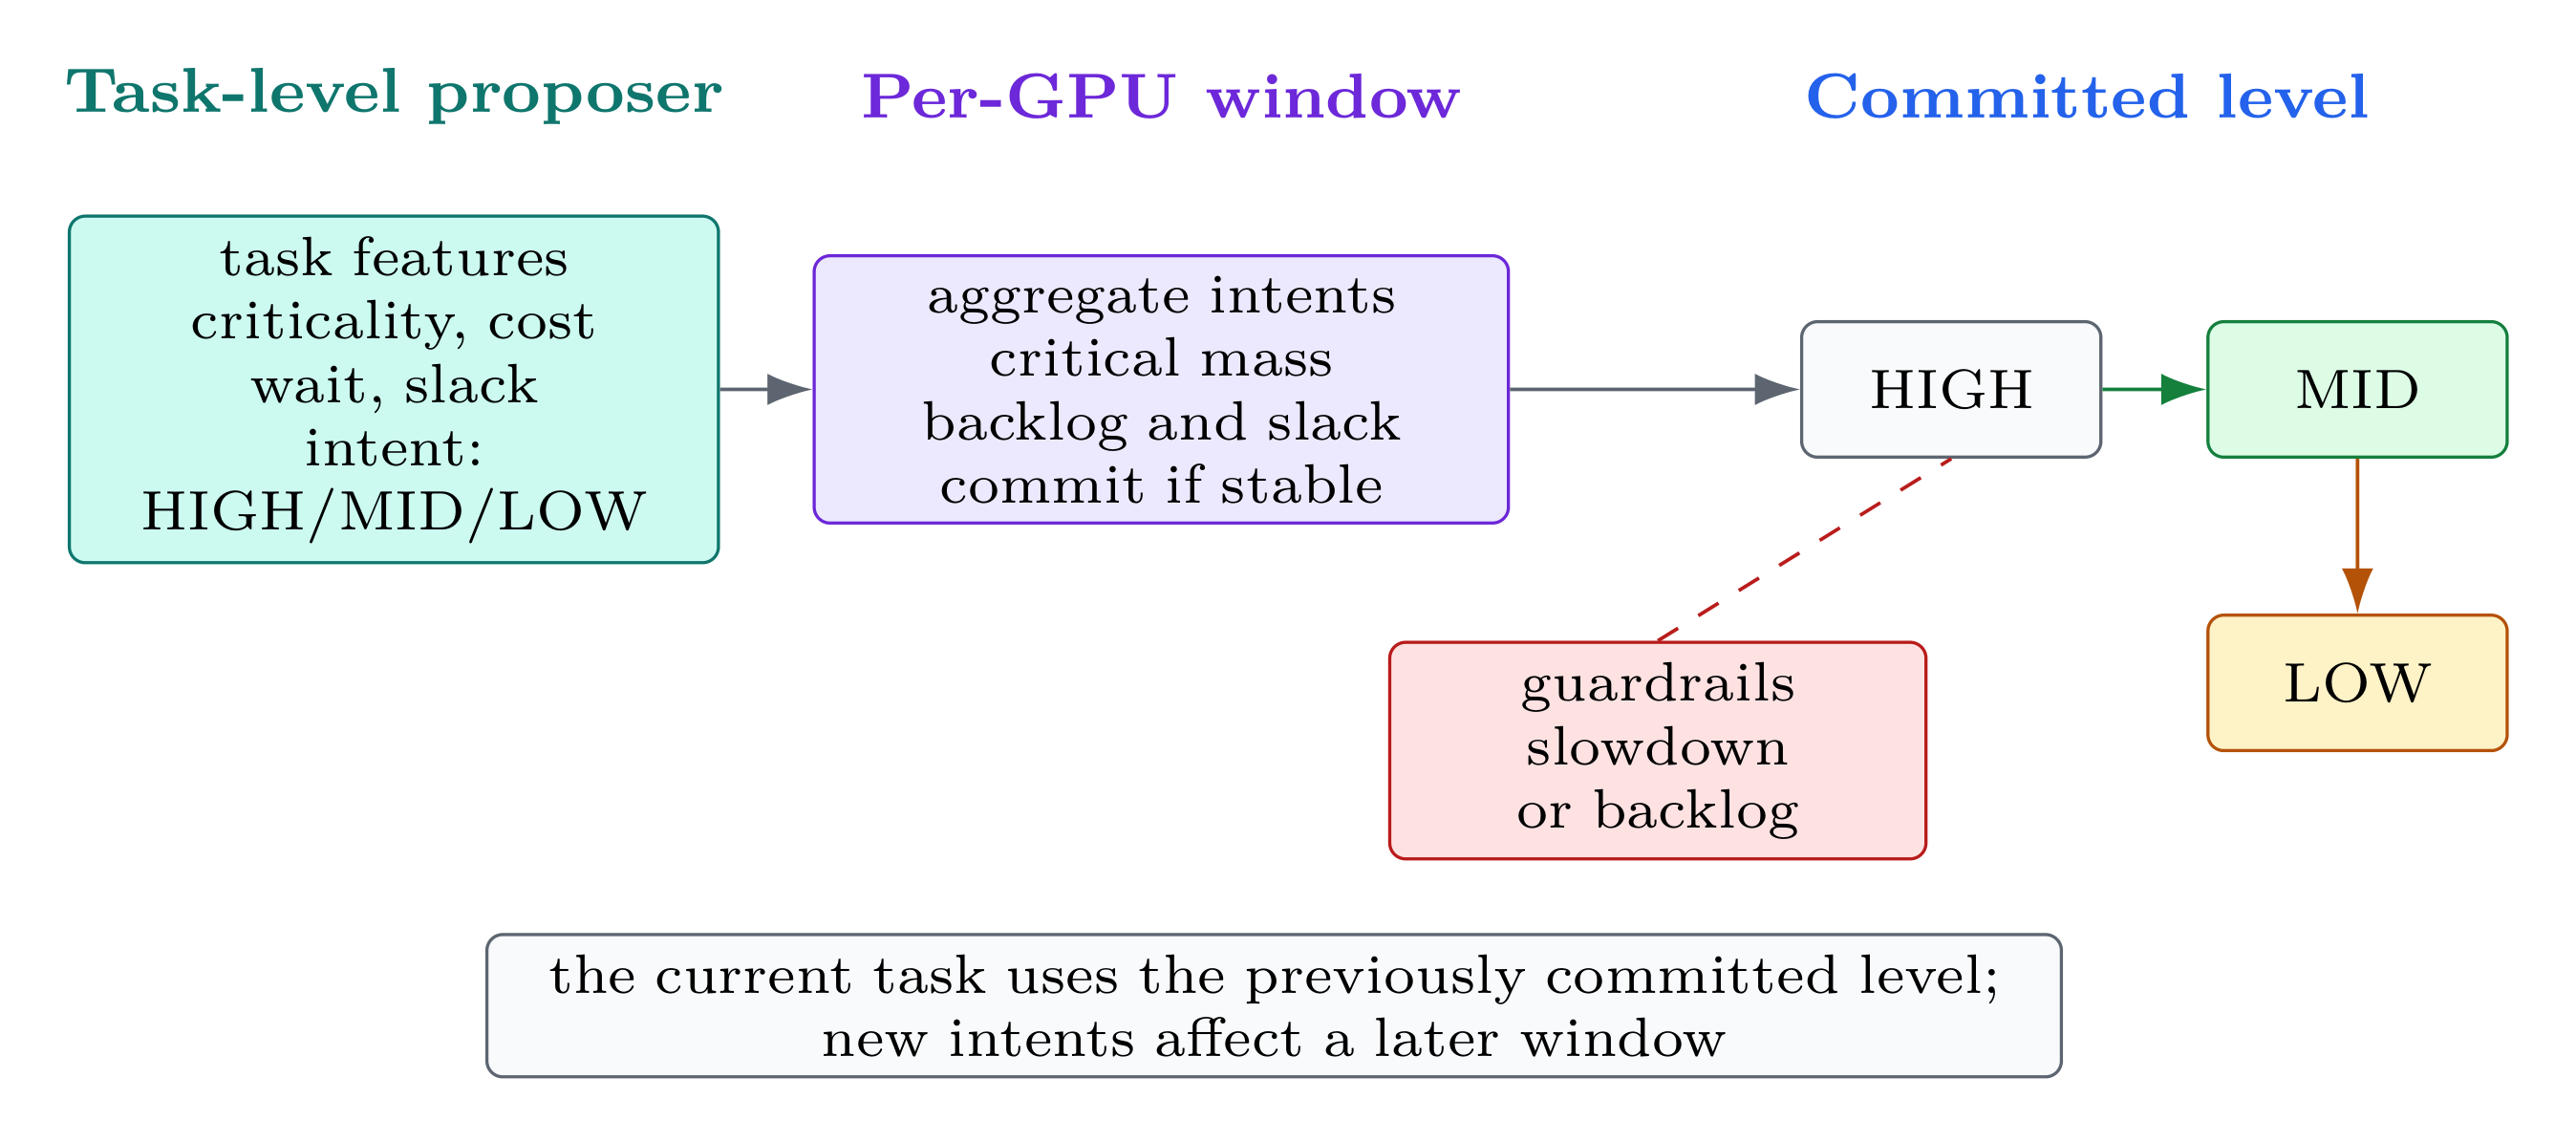
\includegraphics[width=\linewidth,height=0.36\textheight,keepaspectratio]{figures/methods_dvfs_state_machine.png}
\caption{Guarded proposal--commit DVFS state machine. Task-level proposals are accumulated in per-GPU windows, while committed frequency levels change only when lower-frequency eligibility persists and no guardrail forces recovery to high frequency.}
\label{fig:methods-dvfs-state-machine}
\end{figure}%
}
